\documentclass[14pt]{extarticle}
\usepackage[T1]{fontenc}
\usepackage[utf8]{inputenc}
\usepackage{amsmath,amssymb}
\usepackage[russian]{babel}
\usepackage{graphicx}
\usepackage[left=3cm,right=1.5cm,
    top=2cm,bottom=2cm,bindingoffset=0cm]{geometry}
    \usepackage{listingsutf8}
\lstset{columns=fixed,basicstyle=\small,breaklines=true,inputencoding=utf8,keywordstyle=\bfseries\underbar,frame=single,tabsize=2,xleftmargin=20pt,xrightmargin=5pt}
\lstset{language=sql}
\lstset{numbers=left,numberstyle=\small}

\lstset{extendedchars=\true}

\begin{document}

\section*{Лекция 4 (D-схема)}

Так как математические схемы такого вида отражают динамику изучаемой системы, т. е. ее поведение во времени, то они называют­ся D-схемами. 

В простейшем случае обыкновенное дифференциальное уравне­ние имеет вид

\begin{equation}
y'= f(y,t)	
\end{equation}

Наиболее важно для системотехники приложение D-схем в каче­стве математического аппарата в теории автоматического управле­ния. Для иллюстрации особенностей построения и применения D-схем рассмотрим простейший пример формализации процесса функционирования двух элементарных систем различной физической природы: механической $S_m$ (колебания маятника, рис. 2.1, а) и электрической $S_k$ (колебательный контур, рис. 2.1, б).

\begin{figure}[h!]
    \centering
    \includegraphics[scale=1]{d.png}
\end{figure}

Процесс малых колебаний маятника описывается обыкновенным дифференциальным уравнением

\begin{equation}
	m_m l_m^2 \frac{d^2\theta(t)}{dt^2} + m_m g l_m \theta(t) = 0
\end{equation}

где $m_m, l_m$ — масса и длина подвеса маят­ника; g — ускорение свободного падения; в $\theta(t)$ — угол отклонения маятника в момент времени t.

Из этого уравнения свободного колебания маятника можно найти оценки интересующих характеристик. Например, период ко­лебания маятника

\begin{equation}
	T_m = 2 \pi \sqrt{\frac{l_m}{g}}
\end{equation}

Аналогично, процессы в электрическом колебательном контуре описываются обыкновенным дифференциальным уравнением

\begin{equation}
	L_k \frac{d^2q(t)}{dt^2}+\frac{q(t)}{C_k} = 0
\end{equation}

где $L_k,C_k$ — индуктивность и емкость конденсатора; q (t) — заряд конденсатора в момент времени t.

Из этого уравнения можно получить различные оценки харак­теристик процесса в колебательном контуре. Например, период характеристических колебаний

\begin{equation}
	T_k = 2\pi \sqrt{L_kC_k}
\end{equation}

Очевидно, что, введя обозначения $h_0 = m_ml_m^2= L_k, h_1 = 0, h_2 = m_mgl_m= \frac{1}{C_k}, \theta(t) = q(t) = z(t)$ получим обыкновенное дифферен­ циальное уравнение второго порядка, описывающее поведение этой замкнутой системы:

\begin{equation}
h_0 \frac{d^2z(t)}{dt^2} + h_1 \frac{dz(t)}{dt} + h_2 z(t) = 0	
\end{equation}

Где h0, h1, h2 — параметры системы; z(t) — состояние системы в момент времени t.

Таким образом, поведение этих двух объектов может быть исследовано на основе общей математической модели (2.9). Кроме того, необходимо отметить, что поведение одной из систем может быть проанализировано с помощью другой. Например, поведение маятника (системы $S_m$) может быть изучено с помощью электричес­кого колебательного контура (системы $S_k$).

\newpage

\section*{Лекция 13}

\subsection*{Основы GPSS}

GPSS (General Purpose Simulation System) - обещецелевая система моделирования, как и любой другой язык содержит словарь и грамматику, с помощью которых могут быть разработаны точные модели (системы массового обслуживания). Существует множество версий, находится в общем доступе. GPSS построен в предположении, что модели сложной дискретной системы является описание ее элементов и логических правил их взаимодействия. Для определения класса моделируемых систем выделяют конечный набор абстранных элементов, назваемых объектами. Набор логических правил также ограничен (описывается стандартными операциями). Объекты делят на 7 категорий и 14 типов.

Категории:

\begin{enumerate}
	\item Динамическая, ей соответсвует тип transact 
	\item Операционная, ей соответствуют блоки
	\item Аппаратная — тип устройства памяти, ключи
	\item Вычислитель — тип функции, переменные. Среди переменных выделяются арифметические и булевские
	\item Вычислитель — тип функции, переменные. Среди переменных выделяются арифметические и булевские
	\item Запоминающие — ячейки, матрицы ячеек
	\item Группирующие — списки пользователя, группы
\end{enumerate}

Чтобы облегчить переход от алгоритма к программе существует хорошо проработанная…

Основой пакета являются программы, описывающие функционирование выделенного конечного набора объектов и специальная диспетчирезирующая программа, она называется симулятор. Выполняет следующие функции: 

\begin{itemize}
	\item обеспечение заданного программистом маршрута, продвижение динамических объектов (транзакты, сообщения)
	\item планирование событий, происходящих в модели только через время 
	\item регистрация статистической информации 
	\item продвижение модельного времени
\end{itemize}

\subsection*{Категории}

Динамическими объектами являются транзакты, которые представляют собой единицы исследуемых потоков. Они производят ряд действий, продвигаясь по фиксированной структуре. (Структура - совокупность других объектов). 

Операционные объекты — это блоки, задающие логику функционирования модели, определяют пути продвижения транзакта между объектами аппаратной категории.

Объекты аппаратной категории — это абстрактные элементы: устройства памяти, ключи — на которые может быть декомпозирована оборудование реальной системы. Воздействуя на эти объекты, транзакты могут изменять их состояния (влиять на параметры других…)

GPSS описывая каждый объект аппаратной категории требуется ДВА оператора(?): войти в устройство и выйти из него

Вычислительный служит для описания таких ситуаций в процессе моделирования, когда связи между компонентами наиболее просто и компактно выражаются в виде выражения, а выражение строится из переменных и функций. Функции в GPSS имеют свои особенности. Для описания функции либо обращаемся к стандартным (каждая функция задает распределение или плотность) с помощью пар чисел, надо задать тип функции.

GENERATE 7, 3 - равномерное распределение, будут порождаться в диапазоне от 4 до 10 (7+- 3). В качестве модификатора используется интервал. Если используется функция:

GENERATE 3, FN\$XPDES


Здесь модификатором является функция и будет не сложение, а умножение!!! Если написана 3, то умножать надо на значение функции. При умножении получается дробное число и округляется до целого. Получаются нули. Что делать? Масштабировать. 

Статистичекие объекты - очереди и таблицы, оценивают характеристики поведения системы.

В процессе моделирования одни объекты взаимодействуют с другими в результате чего происходит изменение атрибутов и преобразование их значений. Это преобразование называется событием в языке GPSS. Значение атрибута может быть либо арифметическим, либо логическим. Большинство атрибутов не доступны пользователю. Те атрибуты, которые необходимо отрисовать, называются стандартными числовыми атрибутами. Что это за имена? Это имена тех стандартных функций, которые принадлежат … атрибуту. 

При программировании GPSS каждое собственное имя должно быть не менее 5 символов. Это страховка, что мы точно не попадем в стандартный атрибут

\subsection*{Принцип построения и организации}

Имеются два основных типа объекта: транзакты и блоки. Практически все изменения состояния модели системы происходит в результате входа транзакта в блоки и выполнение блоками своих функций. Что связано с блоками? Операционные блоки (они изменябт процесс моделирования), блоки вывода и печати промежуточных результатов, команды управляющие процессом моделирования, команды управляющие редактированием результатов, блок уничтожения транзактов.

Транзакт это любой динамический объект. Может быть физическим.

Основным атрибутом любого транзакта являются его параметры. Значение параметров может быть присвоено блоком asign (?). Количество транзактов каждому параметру от 0 до 1020. Кроме параметров могут быть приоритеты.

Существует такое понятие как транзактные … . Она обозначается как стандартный числовой атрибут m1, определяет интервалы времени.

\subsubsection*{Классификация блоков}

У каждого блока имеется два стандартных числовых атрибута: W - счетчик входов в блок, содержит номер текущего транзакта и N - общий счетчик транзатов, поступивших в блок. Эти два параметра могут быть обнулевы двумя управляющими командами clear и reset.

Классифицируем по назначению

\begin{enumerate}
	\item Блоки, осуществляющие модификацию атрибутов транзакта
	 \begin{enumerate}
		\item временная задержка (блок ADVANCE)
		\item генерация и уничтожение транзактов (блоки GENERATE, SPLIT. SPLIT получает N копий данного транзакта, таким образом блок SPLIT порождает N+1 транзакт) (TERMINATE, ASSEMBLE) 
		\item синхронизация движения нескольких транзактов (MATCH и GATHER)
		\item изменение параметров транзактов (ASSUGN, INDEX, MAC)
		\item изменение приоритета (PRIORITY)
	\end{enumerate}
	\item Блоки, изменяющие последовательность передвижения транзакт
	\begin{enumerate}
	\item блоки передачи управления (TRANSFER, LOOP, TEST, GATE)	
	\end{enumerate}
	\item Блоки, связанные с группирующей категорией (JOIN, REMOVE, scan)
	\item Блоки, сохраняющие необходимые значения для дальнейшего использования (SETVALUE, MSETVALUE)
	\item Блоки, организующие использование объектов аппаратной категории 
	\begin{enumerate}
	\item устройства
	\item FVAL, FUNVAL
	\item ENTER, LEAVE
	\item ключи - LOGIC
	\end{enumerate}
	\item Блоки, обеспечивающие получение статистических результатов (QPAD, TABLE, QUEUE, DEPART, TABULATE)
	\item Специальные блоки  (HELP, TRACE, UNTRACE)
	\item Блоки для организации цепей (LINK, UNLINK)
	\item Вспомогательные блоки (REPORT, LOAD, SAVE)
\end{enumerate}

\begin{figure}[h!]
    \centering
    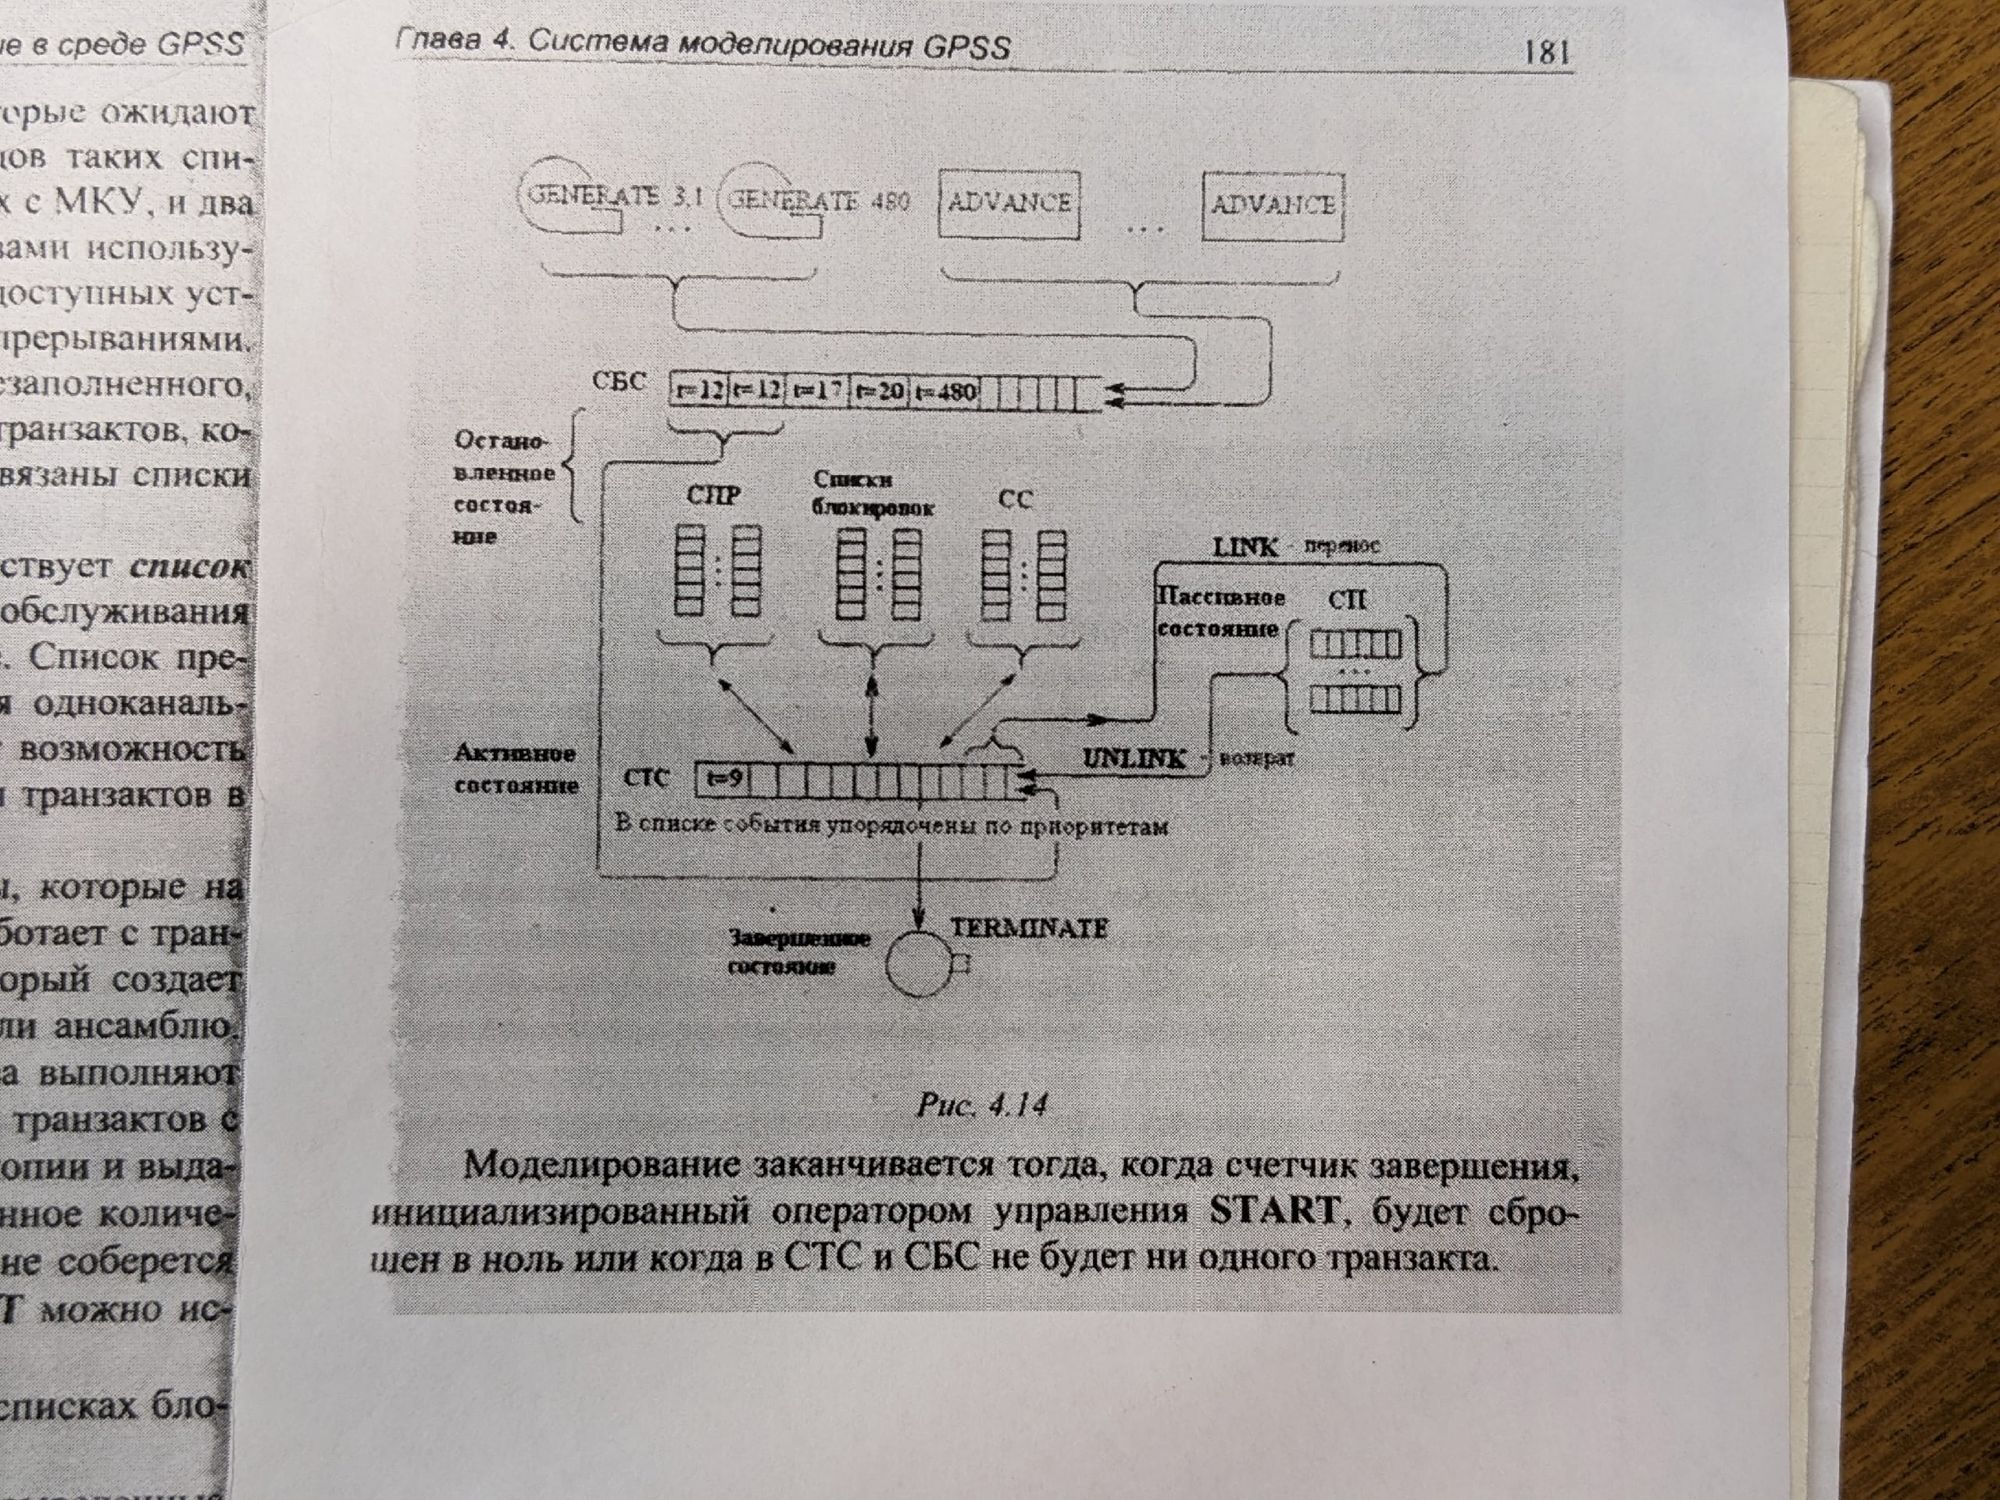
\includegraphics[scale=0.2]{gpss.jpg}
\end{figure}

\newpage

В системе GPSS интерпретатор поддерживает сложные структуры организации списоков с целью уменьшения затрат компьютерного времени на просмотр списка. Система GPSS ведет два основных списка: список текущих событий, куда входят все события, запланированные на текущий модельный момент времени. Интерперататор просматривает в первую очередь этот список и пытается переместить по модели те транзакты, для которых выполняются условия. Если таких транзактов нет, то переходим к просмотру будущих событий, и уже из него снова формируем список текущих событий. 

В начальный момент (как только идентифицировали, что программа на GPSS и включили интерпретатор) обращаемя ко всем блоком generate. Каждый из этих блоков планирует момент появления транзактов и заносит их в СБС, после чего интерператор обращается к списку текущих событий. На первый момент в СТС ничего, интерпретатор рассматривает СБС и выбирает из него все транзакты, запланированные на ближайший момент времени, а затем интерпретатор начинает двигать транзакт по соответсвующим блокам модели. Если уперся в блок адванс (задержка), то он остается в списке текущих событий на время задержки. Если необходимо посмотреть списки событий, то есть специальное окно блоков событий.  

Кроме двух основных списков существует список прерываний, содержащий прерванные во время обслуживания транзакты, как правило используется для организации обслуживания одноканальных устройств по абсолютным приоритетам. 

Список синхронизаций содержит транзакты, которые на данный момент сравниваются. Работает со списком транзактов, созданных блоком split. Именно этот блок создает копии транзактов, принадлежащих одному … . Блок split можно использовать многократно. Синхронизируем с помощью блока match, собираем все копии и один общий - assemble, … собирает и задерживает копии до тех пор, пока не соберет столько, сколько нужно. 

Моделирование заканчивается тогда, когда счетчик завершения инициализированный управляющим оператором старт будет сброшен в ноль или СТС и СБС пусты.

\newpage
\section*{GPSS}

\subsection*{Построение выражений в языке GPSS}

GPSS World поддерживает широкое использование выражений. Они могут использоваться в PLUS-процедурах или в операторах GPSS (если заключены в скобки). Выражения могут выполнять простые вычисления, вызывая процедуры, которые выполняют операции математического характера или операции над строками, выборку возможных распределений или осуществляют реализацию пользовательских алгоритмов, включая файлы ввода-вывода.

Элементы выражений – это основные стандартные блоки выражений, которые, в свою очередь, могут использоваться в полях операндов операторов GPSS и процедурах PLUS.

Элементами выражений могут быть:

\begin{enumerate}
	\item строковые константы, например "Go to metka";
	\item вещественные константы, например 201.6;
	\item целые константы, например 17;
	\item имена, например Kanal;
\end{enumerate}

Арифметические целые переменные определяются с помощью оператора VARIABLE (Переменная). Перед оператором VARIABLE в поле меток ставит ся символьное или числовое имя переменной (идентификатор), а в поле пере менных пишется арифметическое выражение, определяющее данную перемен ную, например: 
19 VARIABLE Q2 + 3

Каждый раз при обращении к арифметическим переменным V19 их значения будут рассчитываться по приведенным выше выражениям, составляю щие которых в процессе моделирования могут менять свои значения.

Вычислительные выражения представляют собой комбинацию математических операторов, библиотечных функций, стандартных числовых атрибутов и кон стант, которые удовлетворяют правилам элементарной алгебры. Они вычисляют ся согласно иерархии операторов, перечисленных выше, и в направлении слева направо. Порядок вычисления можно изменить с помощью круглых скобок, как это делается в любом алгебраическом выражении.

Операторы системы GPSS определяют тип данных непосредственно перед тем, как операция применяется. Поэтому нет необходимости беспокоиться о ти пах данных при создании PLUSвыражений. Выражения могут оцениваться в числовой или строковой формах. Когда выражение оценивается в числовой фор ме, строковый результат преобразуется к его числовому эквиваленту, основанно му на числах, с которых начинается строка. Строка, начинающаяся не с цифры, преобразуется к числовому нулю. Точно так же, когда выражение оценивается как строка, любой числовой результат преобразуется к строковому эквиваленту.

\subsection*{Графические возможности gpss (графики СЧА и гистограммы по таблицам) OR Table, tabulate}

\subsubsection*{Построение графика}

Window -> Simulation Window -> Plot Window

\begin{figure}[h!]
    \centering
    \includegraphics[scale=0.8]{plot1.png}
\end{figure}

Появляется окно Edit Plot Window

Здесь,

label название очереди на графике
\$KASSIRU — текущая длина очереди с именем KASSIRU см. стандартные численные атрибуты.
Title — общее название графика
Time Range — время моделирование
Min value и Max value — минимальное и максимальное значение очереди по оси Y (вертикальная ось)

\newpage

Нажимаем Plot и Memorize

\begin{figure}[h!]
    \centering
    \includegraphics[scale=0.5]{plot2.png}
\end{figure}

Далее, значения появляются в полях Memorized Expression и Window Contents, нажимаем Ок

\begin{figure}[h!]
    \centering
    \includegraphics[scale=0.7]{plot3.png}
\end{figure}

\newpage

Отображается пустая область для графика

\begin{figure}[h!]
    \centering
    \includegraphics[scale=0.4]{plot4.png}
\end{figure}

Затем переходим на вкладку Command -> START, Задаем значение 100 и жмём Ок



В итоги получается график очереди клиентов к кассиру и как видно из графика очередь больше одного человека за длительный промежуток времени, что является отказом в одноканальной СМО.

\begin{figure}[h!]
    \centering
    \includegraphics[scale=0.4]{plot7.png}
\end{figure}

\subsubsection*{Table, tabulate}

Статистические таблицы используются для получения частотных распределений определенных аргументов, которыми могут быть некоторые СЧА (например, времени задержки транзакта в модели в целом или в отдельных ее частях; длин очередей; содержимого памяти и т. д.).

\begin{lstlisting}
	num TABLE A, B, C, D, E
\end{lstlisting}

где num – имя или номер таблицы (совпадает с полем А блока TABULATE A,B);

\begin{enumerate}
	\item А – поле, в котором может быть записан либо аргумент таблицы, т.е. заносимая в таблицу величина и аргумент таблицы может сопровождаться знаком «-» (минус), либо признаки режима формирования данных в таблице: режим IA – ПРОМЕЖУТОЧНЫЙ ИНТЕРВАЛ; режим RT – ИНТЕНСИВНОСТЬ ПРИХОДА);
	\item B – верхняя граница нижнего интервала;
	\item C – ширина интервала;
	\item D – число интервалов;
	\item E – интервал времени ( только для RT — режима).
\end{enumerate}

При входе транзакта в блок TABULATE, которой ссылается на таблицу num, аргумент А этой таблицы вычисляется и заносится в эту таблицу. При этом если за операндом А стоит знак «-«, то в таблицу заносится разность двух соседних значений табулируемой величины. Если в поле А указан режим IA, в таблицу заносится интервал времени между приходом двух транзактов в блок TABULATE.

информация о гистограмме накапливается посредством попадания транзакта в блок:

\begin{lstlisting}
	TABULATE A, B
\end{lstlisting}

где А – имя или номер таблицы, B – вес, указывающий, сколько раз значение должно быть занесено во взвешенную таблицу (по умолчанию В=1).

Функция – стандартный числовой атрибут, название и численная зависимость, обозначаемые в виде FN\$name. Описывается пользователем в виде численной зависимости от другого СЧА. Два основных типа – дискретные и непрерывные.

Пример: 

Дискретная функция:

\begin{lstlisting}
	KL1 FUNCTION S$MEM,D3
	5,12,/9,20/12,6
\end{lstlisting}

Первая строка описания функции должна содержать метку функции в поле метки, слово FUNCTION в поле операции и два операнда в поле операндов. Первый операнд является обозначением того СЧА, который выбран в качестве аргумента функции. В данном примере это S\$MEM – количество занятых единиц памяти MEM. Второй операнд состоит из буквы D, обозначающей, что данная функция дискретная, и из числа точек, которыми задается график функции. Координаты точек, задающих график, записываются в последующих строках описания функции. Из примера видно, что каждая точка задается парой координат, разделенных запятой, причем вначале указывается абсцисса точки, потом ордината. Координаты разных точек разделяются косой чертой. Функция может задаваться любым числом точек. Запись координат точек начинается с 1-й позиции строки и может быть продолжена на последующих строках.

\subsection*{Методика отладки в GPSS}

Для пошагового выполнения модели с целью ее отладки можно воспользоваться командой $STEP A$

Операнд в поле A команды задает количество входов активного транзакта в блоки, которое производится при каждом выполнении команды. Обычно этот операнд равен 1, и каждое выполнение команды STEP приводит к продвижению активного транзакта к следующему блоку. Отладку с использованием команды STEP удобно проводить, находясь в окне блоков. Также можно посмотреть значения выражений через гуи


\begin{figure}[h!]
    \centering
    \includegraphics[scale=0.7]{blocks.png}
\end{figure}


Чтобы остановить процесс моделирования можно ввести команду HALT (Интерактивные команды HALT и SHOW выполняются в момент их ввода, а другие команды ставятся в очередь. Они помещаются в конце списка команд, ко торые еще не были закончены к моменту ввода.)

Для продолжения моделирования после прерывания следует ввести в командную строку команду CONTINUE (продолжить). GPSS имеет в своем составе развитые средства отладки, доступ к которым осуществляется из пункта главного меню «Window → Simulation Window» GPSS реализует пошаговую отладку модели с одновременным отображением процесса перемещения транзактов между блоками ИМ в окне «BLOCK ENTITIES». Для этого в главном меню необходимо выбрать пункт «Window → Simulation Window → Block Window» Для управления процессом моделирования в панели инструментов окна «BLOCK ENTITIES» предусмотрены кнопки «Continue», «Halt» и «Step»

\subsection*{Визуальные средства отображения всякого о модели в процессе работы программы в GPSS}

Для наблюдения за процессом моделирования и действием на него команд на этапе тестирования и верификации используются девять графических окон. Окна подразделяются по типам объектов:

\newpage

блоки

\begin{figure}[h!]
    \centering
    \includegraphics[scale=0.7]{blocks.png}
\end{figure}



выражения

\begin{figure}[h!]
    \centering
    \includegraphics[scale=0.7]{expressions}
\end{figure}

устройства

логические ключи

матрица

\newpage

график


\begin{figure}[h!]
    \centering
    \includegraphics[scale=0.7]{plot.png}
\end{figure}

очереди

\begin{figure}[h!]
    \centering
    \includegraphics[scale=0.7]{queue.png}
\end{figure}

ячейки памяти

таблицы

\begin{figure}[h!]
    \centering
    \includegraphics[scale=1]{table.png}
\end{figure}

Окно блоки показывает выход тразактов в блоки. Оно позволяет с помощью мыши или клавиатуры устанавливать и удалять контрольные точки и визуально отслеживать передвижение транзактов.Окно выражения предназначено для наблюдения за изменениями любого количества Plus-выражений.

С помощью окна график одновременно можно наблюдать любое количество многоцветных графиков.Окно таблица представляет собой динамическую гистограмму, полезную для наблюдения за сбором данных, поиска выбросов и оценки сходимости к порождающему вероятностному распределению.

Окна блоки, устройства, логические ключ, очереди, ячейки, памяти имеют подробный обзор и общий обзор. Открываются они всегда с подробным образом.


\subsection*{Управляющие блоки}

START A, B, C, D

SIMULATE A 

RMULT

RESET

CLEAR

\subsection*{Блоки SEIZE и RELEASE}

SEIZE

RELEASE

\subsection*{Блоки синхронизации транзактов}

MATCH А

ASSEMBLE А

GATHER A


\subsection*{Блоки аппаратной категории GPSS: PREEMPT и RETURN}

PREEMPT A

RETURN A

\subsection*{Блоки изменения параметров транзактов в GPSS}

ASSIGN A,B

ALTER

MARK

\subsection*{Блоки SPLIT/ASSEMBLE}

SPLIT

ASSEMBLE

\subsection*{Язык GPSS. Блоки. Объекты языка}

Lection 13

\subsection*{Язык GPSS. Блоки создания и уничтожения транзактов}

GENERATE

TERMINATE

\subsection*{Язык GPSS. QUEUE, RELEASE}

В GPSS объекты типа "очередь" вводятся для сбора статистических данных. Статистика об очередях собирается в моменты входа транзакта в блок QUEUE (вход в очередь) или в блок DEPART (выход из очереди).

QUEUE!!

Когда сообщение входит в блок QUEUE, то ищется очередь с именем, определенным операндом А. Если необходимо, очередь создается

Поскольку к очереди добавляются единицы, а не сами сообщения, не составляется список членов очереди. Сообщения в этот же момент условного времени пытаются перейти к следующему блоку.

Поскольку очередь обычно используется для измерения времени ожидания, за блоком QUEUE обычно следуют такой блок как SEIZE, который может задержать сообщение.

Одно и то же сообщение может одновременно увеличить длину нескольких очередей, т.е. сообщение может войти в несколько блоков QUEUE перед тем, как войти в соответствующие блоки DEPART.

Значение текущей длины очереди хранится в СЧА Q\$<имя очереди>.

RELEASE!!

Транзакты в GPSS перемещаются от блока к блока. Если в какой-то момент транзакт занимает одноканальное устройство (ОКУ), то он должен войти в соответствующий блок, описывающий ОКУ.

Для SEIZE:

\begin{enumerate}
	\item Если ОКУ уже используют, то транзакт встать в очередь и должен ждать, пока он освободится.
	\item Если ОКУ не используется, то транзак войдёт в блок, а статус ОКУ изменится на «занят».
\end{enumerate}

RELEASE соответственно переводит статус ОКУ в состояние «свободен». В качестве параметров обоим блокам передаётся имя ОКУ.

Для реализации задержек во времени в GPSS применяется блок ADVANCE (продвигать). Этот блок продвигает часы модельного времени на некоторое значение, но фактически он осуществляет задержку продвижения транзакта в течение некоторого интервала времени.

Формат записи блока ADVANCE:

ADVANCE

\subsection*{Язык GPSS. Объекты запоминающей категории, ячейки}

Объекты запоминающей категории обеспечивают обращения к сохраняемым значениям. Ячейки сохраняемых величин и матрицы ячеек сохраняемых величин используются для сохранения некоторой числовой информации.

Любой активный транзакт может произвести запись информации в эти объекты. Впоследствии записанную в эти объекты информацию может считать любой транзакт. Матрицы могут иметь до шести измерений.

Ячейки используются для записи и хранения в процессе моделирования текущих значений СЧА.

Занесение информации в ячейку производится блоком SAVEVALUE,имеющим формат

SAVEVALUE

MSAVEVALUE

\subsection*{Язык GPSS. Ячейки, матрицы ячеек}

SAVEVALUE и ячейки

Наряду с ячейками в моделях можно использовать матрицы ячеек.В отличие от простых ячеек матрицы перед использованием должны быть описаны. Для описания матрицы применяется строка описания матрицы.

MSAVEVALUE

\newpage

\section*{Основные блоки GPSS}

\subsection*{START}

Задание количества заявок

\begin{lstlisting}
	START A,B,C,D
\end{lstlisting}

Поле A содержит целое число, задающее начальное значение счетчика завершений (количество заявок) . В поле B может быть записано ключевое слово NP – признак подавления формирования отчета по завершении моделирования. Если поле B пусто, то формируется отчет со стандартной статистической информацией обо всех объектах модели (как в лабах). Поле C не используется, а поле D может содержать 1 для включения в отчет списков текущих и будущих событий. Если поле D пусто, то выдача в отчет содержимого этих списков не производится.


\subsection*{SIMULATE}

Установка предела времени симуляции

\begin{lstlisting}
	SIMULATE A
\end{lstlisting}

устанавливает предел реального времени, отводимого на прогон модели. Это время (в минутах) задается в его единственном операнде A. Если прогон не завершится до истечения указанного времени, то он будет принудительно прерван с выдачей собранной статистики в отчет. Оператор размещается перед оператором START


\subsection*{RMULT}

Установка начальных значений для генераторов случайных величин

\begin{lstlisting}
	RMULT A,B,C,D,E,F,G
\end{lstlisting}

Оператор RMULT (установить значения генераторов) позволяет перед началом прогона установить начальные значения ГСЧ RN, определяющие генерируемые ими последовательности. Поля A÷G оператора могут содержать начальные значения генераторов соответственно RN1÷RN7, задаваемые числовыми константами. Начальные значения генераторов, не установленные операторами RMULT, совпадают с номерами генераторов.


\subsection*{RESET}

СБрос статистики

\begin{lstlisting}
	 RESET
\end{lstlisting}

Оператор RESET (сбросить) (сброс статистики) сбрасывает всю информацию, накопленную в процессе прогона модели. При этом состояния аппаратных, динамических и запоминающих объектов, а также генераторов, сохраняются, и моделирование возобновляется с новым сбором статистики. Оператор не имеет операндов.

\subsection*{CLEAR}

Сброс симуляции

\begin{lstlisting}
	CLEAR
\end{lstlisting}

Оператор CLEAR (очистить)(сброс модели) очищает модель, подготавливая ее к повторному прогону. При этом сбрасывается вся накопленная в предыдущем прогоне статистика, из модели удаляются все транзакты, и она приводится к исходному состоянию, как перед первым прогоном. Исключение составляют ГСЧ, которые не возвращаются к своим начальным значениям, что позволяет повторить прогон модели на новой последовательности случайных чисел, т.е. организовать независимые прогоны модели. Оператор не имеет операндов.


\subsection*{VARIABLE}

Создание переменной

\begin{lstlisting}
	19 VARIABLE Q2 + 3
\end{lstlisting}

Арифметические целые переменные определяются с помощью оператора VARIABLE (Переменная). Перед оператором VARIABLE в поле меток ставит ся символьное или числовое имя переменной (идентификатор), а в поле пере менных пишется арифметическое выражение, определяющее данную перемен ную, например: 
19 VARIABLE Q2 + 3

\subsection*{TABLE}

Объявление теблицы

\begin{lstlisting}
	num TABLE A, B, C, D, E
\end{lstlisting}

где num – имя или номер таблицы (совпадает с полем А блока TABULATE A,B);

\begin{enumerate}
	\item А – поле, в котором может быть записан либо аргумент таблицы, т.е. заносимая в таблицу величина и аргумент таблицы может сопровождаться знаком «-» (минус), либо признаки режима формирования данных в таблице: режим IA – ПРОМЕЖУТОЧНЫЙ ИНТЕРВАЛ; режим RT – ИНТЕНСИВНОСТЬ ПРИХОДА);
	\item B – верхняя граница нижнего интервала;
	\item C – ширина интервала;
	\item D – число интервалов;
	\item E – интервал времени ( только для RT — режима).
\end{enumerate}

\subsection*{TABULATE}

Помещение информации в таблицу

При входе транзакта в блок TABULATE, которой ссылается на таблицу num, аргумент А этой таблицы вычисляется и заносится в эту таблицу. При этом если за операндом А стоит знак «-«, то в таблицу заносится разность двух соседних значений табулируемой величины. Если в поле А указан режим IA, в таблицу заносится интервал времени между приходом двух транзактов в блок TABULATE.

информация о гистограмме накапливается посредством попадания транзакта в блок:

\begin{lstlisting}
	TABULATE A, B
\end{lstlisting}

где А – имя или номер таблицы, B – вес, указывающий, сколько раз значение должно быть занесено во взвешенную таблицу (по умолчанию В=1).


\subsection*{STEP}

Шаг к следующим блокам (отладка)

\begin{lstlisting}
	STEP A
\end{lstlisting}

Операнд в поле A команды задает количество входов активного транзакта в блоки, которое производится при каждом выполнении команды. Обычно этот операнд равен 1, и каждое выполнение команды STEP приводит к продвижению активного транзакта к следующему блоку. Отладку с использованием команды STEP удобно проводить, находясь в окне блоков. Также можно посмотреть значения выражений через гуи

\subsection*{SEIZE}

Захват устройства



\begin{lstlisting}
	SEIZE DEVICENAME
\end{lstlisting}

\begin{enumerate}
	\item Если одноканальное устройство (ОКУ) уже используют, то транзакт встать в очередь и должен ждать, пока он освободится.
	\item Если ОКУ не используется, то транзак войдёт в блок, а статус ОКУ изменится на «занят».
\end{enumerate}

\subsection*{RELEASE}

\begin{lstlisting}
	RELEASE DEVICENAME
\end{lstlisting}

RELEASE соответственно переводит статус ОКУ в состояние «свободен». В качестве параметров обоим блокам передаётся имя ОКУ.



\subsection*{MATCH}

синхронизирует два транзакта одного семейства

\begin{lstlisting}
	MATCH А
\end{lstlisting}

А - номер сопряженного блока MATCH.

Первый транзакт, достигнув блока MATCH, задерживается в нем до тех пор, пока другой транзакт семейства достигнет сопряженного блока MATCH, указанного в поле А. Во время задержки устанавливается индикатор синхронизации. Он сбрасывается, когда транзакт того же семейства входит в соответствующий блок MATCH.

Пример

\begin{lstlisting}
АA MATCH ВВ
...
ВВ MATCH АА
\end{lstlisting}


\subsection*{ASSEMBLE}

объединение транзактов, принадлежащих одному семейству (или ансамблю)

\begin{lstlisting}
	ASSEMBLE А
\end{lstlisting}

А - число объединяемых транзактов.

Первый транзакт семейства, достигнув блока ASSEMBLE, задерживается в нем до тех пор, пока остальные члены семейства не поступят в этот блок. Когда транзакты, число которых указано в поле А, поступят в этот блок, они будут удалены из модели, а первый прибывший транзакт продолжит движение.

Пример

\begin{lstlisting}
ASSEMBLE 3
\end{lstlisting}

После того, как 3 транзакта одного семейства войдут в блок, один (первый) выйдет из блока и продолжит движение, остальные будут уничтожены.

\subsection*{GATHER}

накапливает транзакты, являющиеся членами семейства

\begin{lstlisting}
	GATHER A
\end{lstlisting}

Транзакты одного семейства задерживаются в блоке GATHER до тех пор, пока их число не станет равным значению поля А. Когда последний транзакт войдет в блок GATHER, все они одновременно выходят из него в том порядке, в котором поступили. Состояние блока GATHER может быть проверено блоком GATE.

Пример

\begin{lstlisting}
GATHER 6
\end{lstlisting}

Транзакты накапливаются в этом блоке до тех пор, пока в нем не соберутся шесть транзактов из одного семейства, после чего все они смогут продолжать движение.

\subsection*{PREEMPT}

переводит устройство в прерванное состояние

\begin{lstlisting}
	PREEMPT A
\end{lstlisting}

Транзакт, попадающий в блок PREEMPT, захватывает устройство, имя которого указано в поле A блока. Если при захвате устройства оно свободно, то транзакт просто занимает устройство, в этом случае блок PREEMPT работает аналогично блоку SEIZE. Если при входе транзакта в блок PREEMPT устройство занято другим транзактом, то в этом случае транзакт входит в блок PREEMPT, а устройство прерывает обслуживание занимающего его транзакта и переключается на обслуживание транзакта, вошедшего в блок PREEMPT. При этом из состояния «занято» устройство переходит в состояние «захвачено». Когда транзакт, захватывающий устройство, освободит его, устройство возобновит прерванное обслуживание другого транзакта и перейдет в состояние «занято».

Пример

\begin{lstlisting}
PREEMPT Р$1
\end{lstlisting}

Если устройство, номер которого задан параметром Р1, не было переведено в состояние прерывания, то транзакт, входящий в этот блок, захватывает его.

\subsection*{RETURN}

\begin{lstlisting}
	RETURN A
\end{lstlisting}

Этот блок используется в паре с блоком PREEMPT. Если транзакт захватил устройство посредством блока PREEMPT, то освободить его он может только в блоке RETURN. Имя освобождаемого устройства задается в поле A блока.

При входе транзакта в блок RETURN снимается прерывание с устройства, которое было прервано этим транзактом. Снятие прерывания должно быть осуществлено тем же транзактом, который вызвал прерывание. Если устройство было занято до прерывания, то прерванный транзакт возвращается на дообслуживание после снятия прерывания.

Пример

\begin{lstlisting}
RETURN 1
\end{lstlisting}

Транзакт снимает прерывание устройства 1.

\subsection*{ASSIGN}

изменяет значение параметра транзакта

\begin{lstlisting}
	ASSIGN A,B
\end{lstlisting}

А - номер изменяемого параметра (+, -);

В - новое значение параметра.

Если за полем А следует знак + или -, то значение поля В соответственно добавля-ется или вычитается из А. Если знаки - или + не указаны, то значение поля В становится текущим значением параметра.


Пример

\begin{lstlisting}
ASSIGN 2,8
\end{lstlisting}

Присваивает параметру 2 значение 8.

\subsection*{ALTER}

Блок изменяет приоритет или параметр выбранных членов группы транзактов.

\begin{lstlisting}
	ALTER  [X]  A,[B],C,D,[E] ,[F],[G]
\end{lstlisting}

\begin{enumerate}
	\item X - Задает операцию сравнения операндов E и F. При выполнении сравнения происходит изменение приоритета или параметров транзактов.
	\item A - Номер или имя группы, члены которой будут проверяться для проведения изменений.
	\item B - Максимальное количество транзактов, атрибуты которых должны быть изменены.
	\item C - Максимальное количество транзактов, атрибуты которых должны быть изменены.
	\item D - Максимальное количество транзактов, атрибуты которых должны быть изменены.
	\item E - Проверяемый атрибут. Параметр транзакта, по которому определяется, должен ли изменяться член группы, или PR, если для определения используется приоритет транзакта
	\item F - Значение, с которым сравнивается операнд Е.
	\item G - Определяет блок для перехода транзакта при выполнении некоторых условий. 
\end{enumerate}

Особенности выполнения.

\begin{enumerate}
	\item Блок всегда принимает транзакты.
	\item Блок ALTER выбирает транзакты из группы транзактов и изменяет один из атрибутов каждого из них. При изменении члена группы транзактов, его атрибуту, определяемому операндом С, присваивается значение, определяемое операндом D.
	\item Если не используется условный оператор и операнды Е или F, то изменяются все транзакты вплоть до предела, заданного операндом В. В этом случае не проверяются  приоритет или параметр для определения, будет ли изменяться атрибут транзакта-члена группы.
	\item При использовании условного оператора и операндов Е и F изменяются все транзакты, для которых выполняется условие сравнения.
	\item Если в качестве условного оператора задано MIN или МАХ то операнд Е определяет, какой атрибут транзакта группы должен сравниваться с минимальным или максимальным значением этого атрибута среди членов группы, Все транзакты, для которых выполняется условие сравнения, изменяются. В этом случае не используется операнд F.
	\item При использовании операнда G, вошедший транзакт переходит в блок, определяемый данным операндом,
\end{enumerate}

\subsection*{MARK}

ставит отметку времени или записывает значение таймера.

\begin{lstlisting}
	MARK A
\end{lstlisting}

А - номер параметра, в который записывается значение таймера абсолютного времени.

Если поле А не используется, отметка времени (время создания транзакта) заменя-ется значением текущего таймера. Если поле А определено, то текущее значение таймера записывается в параметр, указанный в поле А.

\subsection*{SPLIT}

создает копии текущего транзакта

\begin{lstlisting}
	SPLIT A,B,C,D
\end{lstlisting}

\begin{enumerate}
	\item А - число создаваемых копий;
	\item В - следующий блок для копий;
	\item С - параметр для хранения порядкового номера копии;
	\item D - число параметров у каждой копии.
\end{enumerate}

Поле А определяет число копий, которые образуются при входе текущего транзак-та. Эти вновь созданные транзакты по умолчанию идентичны исходному транзакту. Копии входят в блок, указанный в поле В. Исходный транзакт поступает на следующий блок. Параметр поля С используется для задания порядковых номеров копий. Нумерация осуществляется следующим образом. Порядковый номер исходного транзакта увеличивается первым. Если он был равен нулю, при входе транзакта в блок он станет равным единице. Порядковый номер первой копии станет на единицу больше, чем у исходного транзакта Ломера последующих копий также увеличиваются на единицу. Если поле D не задано, копии имеют такое же, как у исходного транзакта число и тип параметров.

Пример

\begin{lstlisting}
SPLIT 4,THERE
\end{lstlisting}

Создает 4 копии вошедшего транзакта и посылает в блок с именем THERE. Исходный транзакт идет на следующий блок.

\begin{lstlisting}
SPLIT 3,Р$1,1,4
\end{lstlisting}

Создает три копии текущего транзакта. Каждая копия будет иметь четыре параметра; порядковый номер указан в параметре 1. Параметр P\$1 будет определять номер следующего блока.

\subsection*{GENERATE}

вводит транзакты в модель

\begin{lstlisting}
	GENERATE A,B,C,D,E,F,G
\end{lstlisting}

\begin{enumerate}
	\item А - среднее значение интервала времени;
	\item В - разброс или модификатор среднего значения(по умолчанию ноль);
	\item С - время появления первого транзакта;
	\item D - общее число генерируемых транзактов;
	\item Е - уровень приоритета каждого транзакта;(от 0 до 127,значение по умолчанию 0);
	\item F - число параметров (по умолчанию 12);
	\item G - тип параметра ( F - полнословный, Н - полусловный - по умолчанию )
\end{enumerate}

Вводит транзакты в модель, посылая их в следующий по порядку блок. Если в поле В не указана Функция, то интервал между поступлением транзактов определяется случайным числом, равномерно распределенным в диапазоне от (А - В) до (А + В). Если поле В является функцией (FN\$), то этот интервал определяется произведением поля А на значение функции, заданной в поле В.

Пример

\begin{lstlisting}
GENERATE 15,3,25
\end{lstlisting}

Генерируются транзакты с интервалом прихода от 12 до 18 единиц времени, пер-вый из которых поступает в момент времени 25 единиц.

\begin{lstlisting}
GENERATE (EXPONENTIAL(1,2,3))
\end{lstlisting}

Генерируются транзакты с интервалом, распределенном по экспоненциальному закону.

\subsection*{TERMINATE}

удаляет транзакт

\begin{lstlisting}
	TERMINATE A
\end{lstlisting}

А - величина, вычитаемая из содержимого счетчика завершений(поле А карты START).

Транзакт удаляется из модели и поступает в пассивный буфер. Если в поле А пробел, воздействия на счетчик завершений не происходит, в противном случае его значение уменьшается на величину, указанную в поле А.

Пример

\begin{lstlisting}
TERMINATE
\end{lstlisting}

Транзакт удален, но значение счетчика завершений не изменяется.

\begin{lstlisting}
TERMINATE 2
\end{lstlisting}

Значение счетчика завершений уменьшается на 2.

\subsection*{QUEUE}

увеличивает длину очереди

\begin{lstlisting}
QUEUE A,[B]	
\end{lstlisting}

В поле А задается номер или имя очереди, к длине которой добавляются единицы. Операнд может быть именем, положительным целым, СЧА.

Поле В определяет число единиц, на которое увеличивается текущая длина очереди. Если поле В пусто, то прибавляется единица.

Когда сообщение входит в блок QUEUE, то ищется очередь с именем, определенным операндом А. Если необходимо, очередь создается.

Поскольку к очереди добавляются единицы, а не сами сообщения, не составляется список членов очереди. Сообщения в этот же момент условного времени пытаются перейти к следующему блоку.

Поскольку очередь обычно используется для измерения времени ожидания, за блоком QUEUE обычно следуют такой блок как SEIZE, который может задержать сообщение.

Одно и то же сообщение может одновременно увеличить длину нескольких очередей, т.е. сообщение может войти в несколько блоков QUEUE перед тем, как войти в соответствующие блоки DEPART.

Значение текущей длины очереди хранится в СЧА Q\$<имя очереди>.

\subsection*{DEPART}

уменьшения длины очереди.

\begin{lstlisting}
	DEPART A,B
\end{lstlisting}

В поле А задается номер или имя очереди, длину которой нужно уменьшить. В поле В задается число единиц, на которое уменьшается длина очереди. Это число не должно превышать текущую длину очереди. Если поле В пусто, длина очереди уменьшается на единицу.

\subsection*{ADVANCE}

задержка

\begin{lstlisting}
	ADVANCE A, [B]
\end{lstlisting}

где А – среднее время задержки на обслуживание (число, СЧА, значение по умолчанию – 0);

В – половина поля допуска равномерно распре­деленного времени задержки (число, СЧА, значение по умолчанию – 0).

Кроме того, тут может быть распределение (как в GENERATE)

\subsection*{SAVEVALUE}

сохраняет значение

\begin{lstlisting}
	SAVEVALUE A,B,C
\end{lstlisting}

\begin{enumerate}
	\item А - номер ячейки;
	\item В - присваиваемое значение;
	\item С - тип ячейки: XF, ХН, XL (по умолчанию XF).
\end{enumerate}

Если за полем А стоит знак " + " или знак " - ", значение поля В, соответственно, прибавляется или вычитается из текущего содержимого ячейки. Если знаки + " или " - " не указаны, то значение поля В записывается в ячейку. Поле С определяет тип ячейки (ХН - полусловная; XF - полнословная; XL - с плавающей точкой).


Пример

\begin{lstlisting}
	SAVEVALUE 4,5
\end{lstlisting}

Поместить значение 5 в полнословную ячейку 4.

\begin{lstlisting}
	SAVEVALUE 2+,Р$3,Н
\end{lstlisting}

Прибавить содержимое параметра 3 к содержимому полусловной ячейки 2.


\subsection*{MATRIX}

Создание матрицы

\begin{lstlisting}
	j MATRIX A B C
\end{lstlisting}

Наряду с ячейками в моделях можно использовать матрицы ячеек.В отличие от простых ячеек матрицы перед использованием должны быть описаны. Для описания матрицы применяется строка описания матрицы.

\begin{enumerate}
	\item j - имя матрицы.
	\item А - неиспользуемое поле (для совместимости с прежними версиями GPSS).
	\item B - количество строк матрицы. Обязателен. Операнд должен быть константой.
	\item С - количество столбцов матрицы. Обязателен. Операнд должен быть константой.
\end{enumerate}


Пример

\begin{lstlisting}
	ARRAY MATRIX ,100,5
\end{lstlisting}

Этот карта определяет матрицу ARRAY, которая имеет 100 строк и 5 столбцов. Этот карта определяет матрицу ARRAY, которая имеет 100 строк и 5 столбцов.
В начальный момент любая матрица содержит только нулевые значения.

Обращение MX\$j(A,B).

\subsection*{MSAVEVALUE}

Запись значения в ячейку матрицы

\begin{lstlisting}
	MSAVEVALUE A,B,C,D
\end{lstlisting}

А - имя или номер матрицы,В - номер строки, С - номер столбца, D - новая величина элемента матрицы

\subsection*{GATE}

вспомогательный блок, проверяющий состояния устройств, памятей, логических ключей

\begin{lstlisting}
GATE_R А,В

\end{lstlisting}

\begin{enumerate}
	\item U - устройство занято;
	\item NU - устройство не занято;
	\item 1 - устройство прервано;
	\item NI - устройство не прервано;
	\item SF - память заполнена;
	\item SNF - память не заполнена;
	\item SE - память пустая;
	\item SNE - память не пустая;
	\item LR - ключ выключен;
	\item LS - ключ включен;
	\item М - транзакт находится в состоянии синхронизации;
	\item MN - транзакт не находится в состоянии синхронизации. 
\end{enumerate}

Если проверяемое условие для объекта, номер которого определяется полем А, выполняется (СЛА "ИСТИНА"), то транзакт входит в блок GATE. Если условие "ЛОЖЬ", то возможны два случая:

\begin{enumerate}
	\item если поле В задано, то транзакт идет в блок, номер которого указан в поле В;
	\item если в поле В пробел, то транзакт ждет в предыдущем блоке, пока не выполнится условие. 
\end{enumerate}


\subsection*{TRANSFER}

изменяет движение транзакта в модели

\begin{lstlisting}
	TRANSFER А,В,С,D
\end{lstlisting}

\begin{enumerate}
	\item А - режим передачи (пробел,.,ALL,BOTH,FN,P,PICK,SBR,SIM); 
	\item В - следующий блок; 
	\item С - следующий блок; 
	\item D - значение индекса, используемое в режиме ALL. 
\end{enumerate}

Транзакт направляется в блок, определяемый в соответствии с режимом передачи, указанным в поле А.

Режимы передачи поля А: 

\begin{enumerate}
	\item Пробел - транзакт передается в блок, определяемый полем В. 
	\item "." - статистический режим; в поле А указано десятичное число, выражающее ероятность перехода в блок С; его дополнение до единицы указывает вероятность перехода в блок В.
	\item ALL - транзакт последовательно пытается перейти в блоки, определяемые значениями В, B+D, B+2D.....C.
	\item BOTH - транзакт последовательно пытается войти в блок В, затем в блок С, до тех пор, пока один из них станет доступным. 
	\item FN - функциональный режим: поле В является номером функции; следующий блок определяется суммой значения этой функции поля С. 
	\item Р - параметрический режим: поле В является номером параметра; следующий блок определяется суммой значения этого параметра и поля С. 
	\item PICK - выборочный режим: блок выбирается с равной вероятностью из блоков с номерами: В, B+l,..., С. 
	\item SBR - режим перехода к подпрограмме: номер текущего блока помещается в параметр, указанный в поле С, а транзакт передается в блок, номер которого указан в поле В. 
	\item SIM - одновременный режим: проверяется одновременное выполнение условий беспрепятственного движения транзактов в задерживающих блоках. Если условие выполняется, транзакт передается в следующий блок, в противном случае транзакт переходит на блок С. 
\end{enumerate}

\subsection*{JOIN}

Блок добавляет активный транзакт в группу транзактов или число к числовой группе 

\begin{lstlisting}
	JOIN A,[B]
\end{lstlisting}

\subsection*{REMOVE}

Блок удаляет активный транзакт из группы транзактов или число из числовой группы.

\begin{lstlisting}
	 REMOVE  [X]  A,[B],[C],[D],[E],[F]
\end{lstlisting}

\subsection*{LOGIC}

Работа логических ключей

Имитация процессов коммутации в GPSS выполняется с использованием логических ключей, имеющих два состояния «Включено» — «Выключено».

\begin{lstlisting}
	LOGIC_r A
\end{lstlisting}

где А — имя логического ключа, r — внутренний оператор, принимающий значения I — переключить, R — выключить, S — включить. При входе транзакта в блок LOGIC происходит срабатывание соответствующего ключа. Ключи не имеют СЧА. Их состояния задаются только стандартными логическими атрибутами:

\begin{lstlisting}
	LS$j — ключ j включен; LR$j — ключ j выключен.
\end{lstlisting}

Можно проверить с помощью GATE


\subsection*{STORAGE}

Память (STORAGE) представляет собой объект GPSS, обладающий определенной емкостью.

Ёмкость памяти задаётся в разделе объявлений GPSS-программы

\begin{lstlisting}
	num STORAGE A
\end{lstlisting}

где num — имя или номер памяти;
А — ёмкость памяти (целое без знака), по умолчанию А = 32767.

\subsection*{ENTER}

Войти в память

\begin{lstlisting}
	ENTER A, B
\end{lstlisting}

\subsection*{LEAVE}

Выйти из памяти

\begin{lstlisting}
	LEAVE A, B
\end{lstlisting}

\subsection*{ANOVA}

Дисперсионный анализ

\begin{lstlisting}
	ANOVA(ResultMatrixName,ReplicateDimension,InteractionLimit)
\end{lstlisting}

Дисперсионный анализ состоит в выделении и оценке отдельных факторов, вызывающих изменчивость среднего значения наблюдаемой случайной величины. С этой целью производится разложение дисперсии наблюденной частичной совокупности на составляющие, порождаемые независимыми факторами. Каждая из этих составляющих получает свою оценку в общей совокупности.

Для проверки значимости факторов оценивают значимость указанных составляющих дисперсии, сравнивая их с так называемой остаточной дисперсией, обусловленной случайным составом частичной совокупности.

\end{document}